\documentclass[t, 14pt, aspectratio=1610]{beamer}
 % align text inside frame to t=top, b=bottom, c=center
 % 8pt, 9pt, 10pt, 11pt, 12pt, 14pt, 17pt, 20pt available as text font
 % select your aspect ratio 4:3=43, 16:9=169, 16:10=1610

\usetheme{Juelich}

%\usetheme{default}
%\usecolortheme{beaver}

\setbeamertemplate{caption}[numbered]
\setbeamertemplate{caption label separator}{:}
\setbeamertemplate{slide counter}[showall]
\setbeamercolor{code}{fg=black,bg=fzjblue!10}
\setbeamercolor{prototype}{fg=black,bg=fzjgreen!20}

\setbeamertemplate{footline}{%
\hfill\usebeamertemplate***{navigation symbols}
\hspace{-1cm}\small\insertframenumber{}/\inserttotalframenumber}


% \setbeamertemplate{footer element1}[default][\insertsection]%

\usepackage{graphics}
\newcommand{\gfxpath}{../images}

\usepackage[ngerman,english]{babel}
%\selectlanguage{ngerman}
\selectlanguage{english}
\usepackage[utf8]{inputenc}
\usepackage[T1]{fontenc}
% =====================================================
%  packages / definitions needed by pandoc
%
\usepackage{xcolor}
\usepackage{fancyvrb}
\usepackage{framed}
\usepackage{longtable}
\usepackage{booktabs}
\usepackage[warn]{textcomp}
% package listings important for code highlighting !
\usepackage{listings}

\providecommand{\tightlist}{%
  \setlength{\itemsep}{0pt}\setlength{\parskip}{0pt}}

%\renewcommand{\emph}[1]{\structure{#1}}

\renewcommand{\thefootnote}{}

% AUTHOR AND TITLE FOR TITLE PAGE
\author[M. Cherti]{Mehdi Cherti}
\institute[JSC]{Cross Sectional Team Deep Learning, Helmholtz AI @ JSC}
\date{2021-05-07}
\title{Day 5: Advanced Generative Adversarial Networks (GANs)}
% \subtitletest{}

%\AtBeginPart{%
%  \subtitle{\partname}
%  \makepart
%  \begin{frame}
%  \frametitle{Outline}
%  \tableofcontents[hideallsubsection]
%  \end{frame}
%}

%\AtBeginSection{%
%  \subtitle{\sectionname}
%  \begin{frame}
%  \frametitle{Outline}
%  \tableofcontents[currentsection]
%  \end{frame}
%}

% -- INCLUDE BACKGROUND GRAPHIC FOR TITLE PAGE
% \titlegraphic{\includegraphics[width=\paperwidth]{../Abbildungen/juwels_cluster_booster_banner}}


\begin{document}
% Titelseite
\fzjset{title page=image}

%\fzjset{title page=text}
\maketitle

%\begin{frame}
%  \frametitle{Outline}
%  \tableofcontents
%\end{frame}

%% pandoc generated slides
\begin{frame}{Generative Models}
\protect\hypertarget{generative-models}{}

\begin{itemize}
\tightlist
\item
  Impressive progress in last years, algorithmic improvements coupled
  with \textbf{large scale training} and \textbf{large models}
\end{itemize}

\center{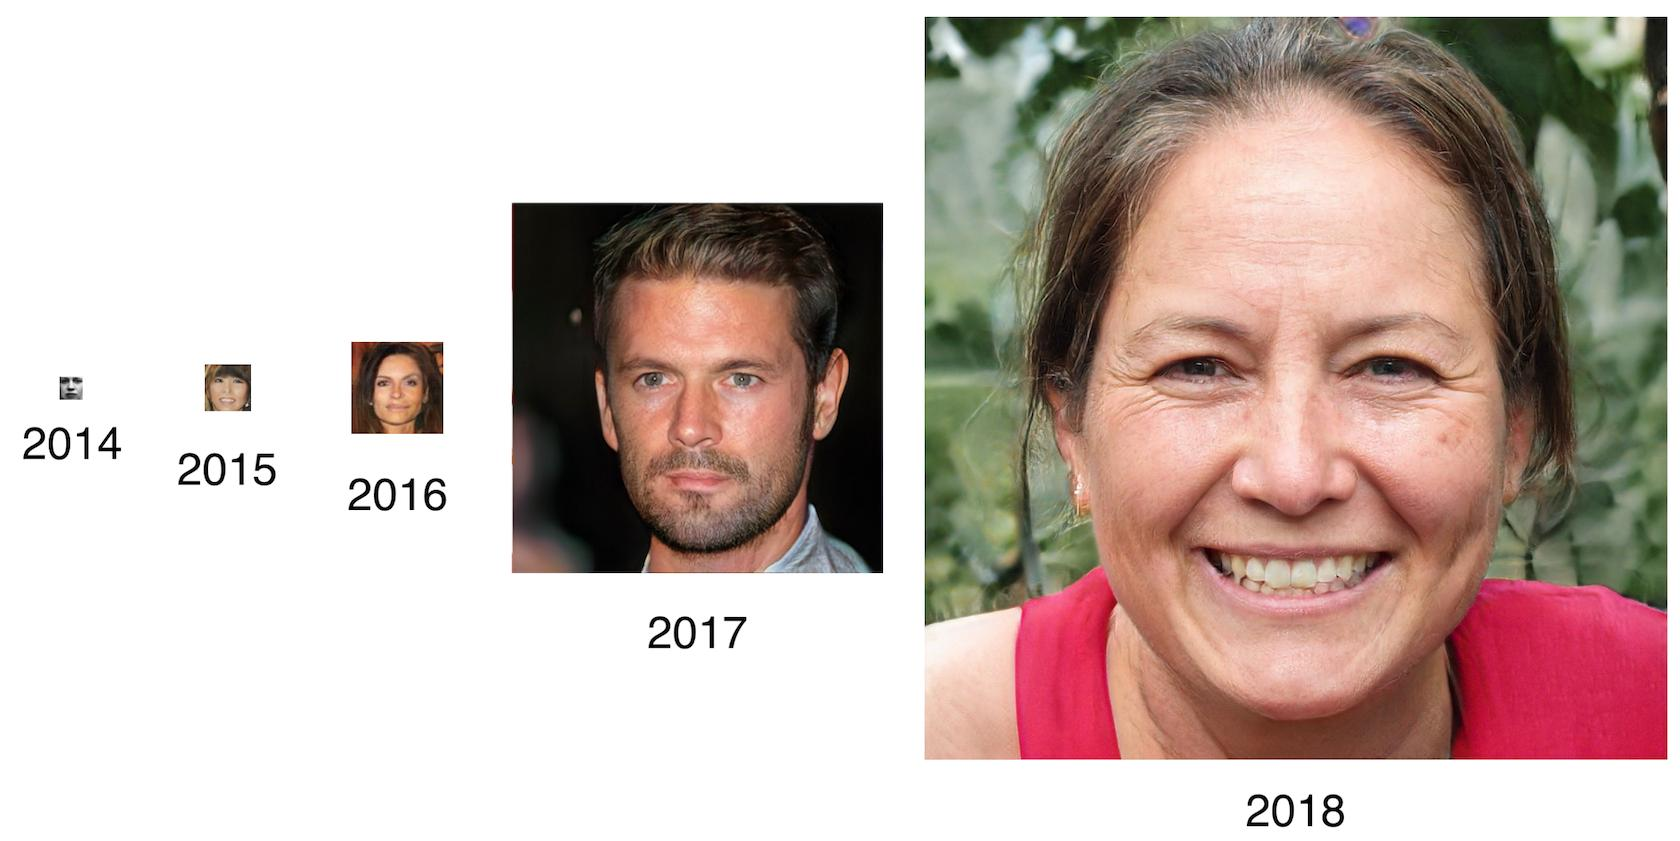
\includegraphics[width=0.7\textwidth]{images/gan_evolution.jpeg}}

(Source: \url{https://bit.ly/3azTV7J})

\end{frame}

\begin{frame}{Generative modeling benefit from scaling: BigGAN}
\protect\hypertarget{generative-modeling-benefit-from-scaling-biggan}{}

\begin{itemize}
\tightlist
\item
  BigGAN (Brock, Donahue, and Simonyan 2019) was the first architecture
  to scale to ImageNet-1K
\item
  Trained on high resolution up to 512x512, and have \textbf{high
  diversity and high quality samples}
\end{itemize}

\center{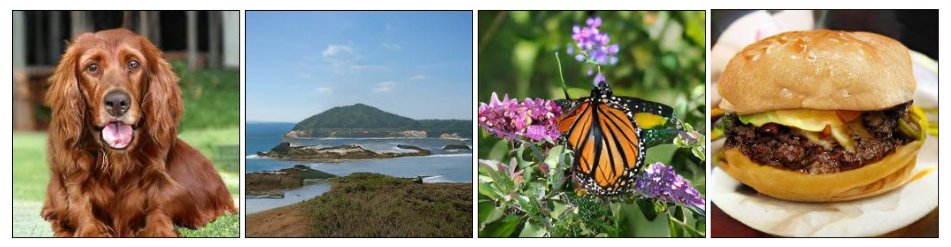
\includegraphics[width=0.8\textwidth]{images/biggan.png}}

\end{frame}

\begin{frame}{Generative modeling benefit from scaling: BigGAN}
\protect\hypertarget{generative-modeling-benefit-from-scaling-biggan-1}{}

\begin{itemize}
\tightlist
\item
  Model much larger than previous works: scaling width and and depth
\item
  Batch size (up to 2048) much bigger than previous works
\item
  Benefit of scaling the model: reach better performance in
  \textbf{fewer iterations}
\end{itemize}

\center{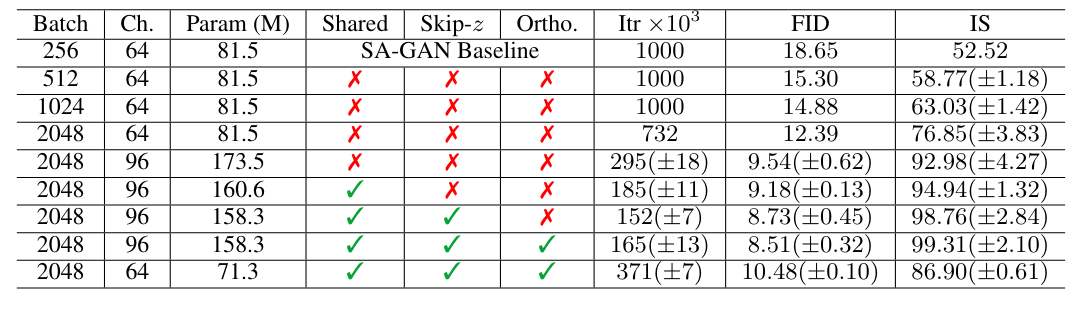
\includegraphics[width=0.8\textwidth]{images/biggan_results.png}}
\center{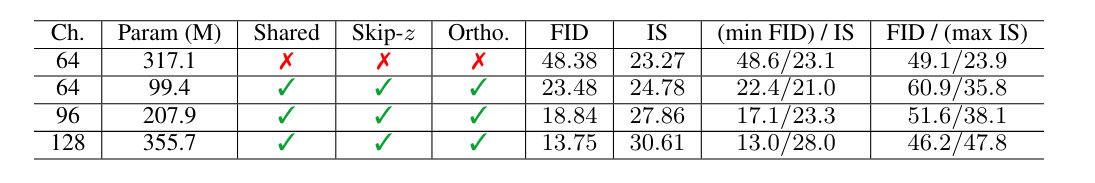
\includegraphics[width=0.8\textwidth]{images/biggan_results_2.png}}

\end{frame}

\begin{frame}{Generative modeling benefit from scaling: BigGAN}
\protect\hypertarget{generative-modeling-benefit-from-scaling-biggan-2}{}

\begin{itemize}
\tightlist
\item
  512x512 resolution model trained on 512 TPUs (TPU v3 pod)
\item
  Training takes between 24 hours and 48 hours for most models
\item
  Results as model size is increased:
  \center{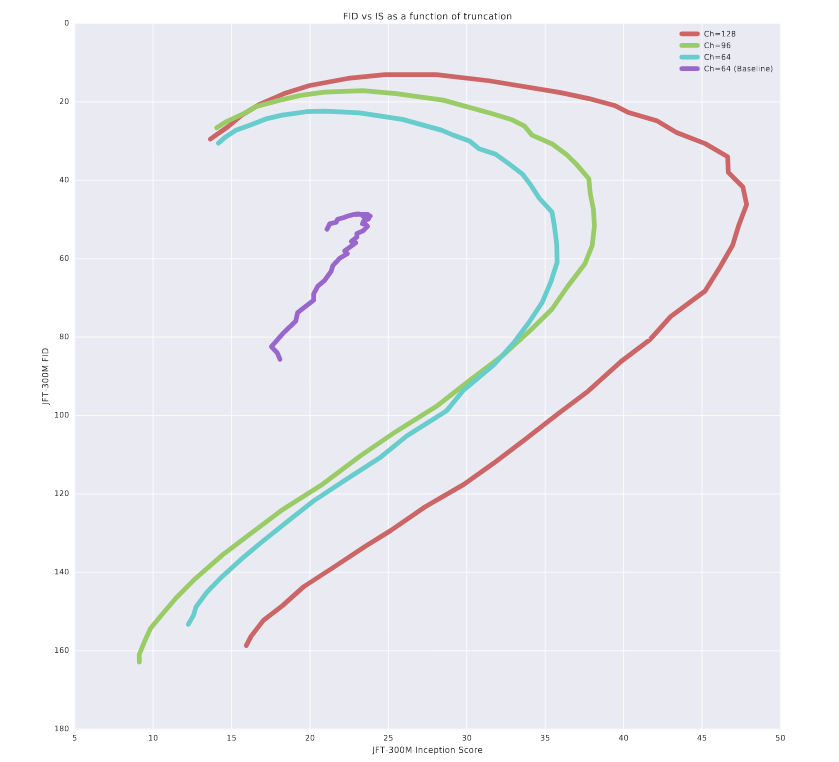
\includegraphics[width=0.40\textwidth]{images/biggan_results_6.png}}
\end{itemize}

\end{frame}

\begin{frame}{Generative modeling benefit from scaling: BigGAN}
\protect\hypertarget{generative-modeling-benefit-from-scaling-biggan-3}{}

\begin{itemize}
\tightlist
\item
  a lot of tuning is necessary in experimentation, before finding the
  good range of hyper-parameters
\end{itemize}

\center{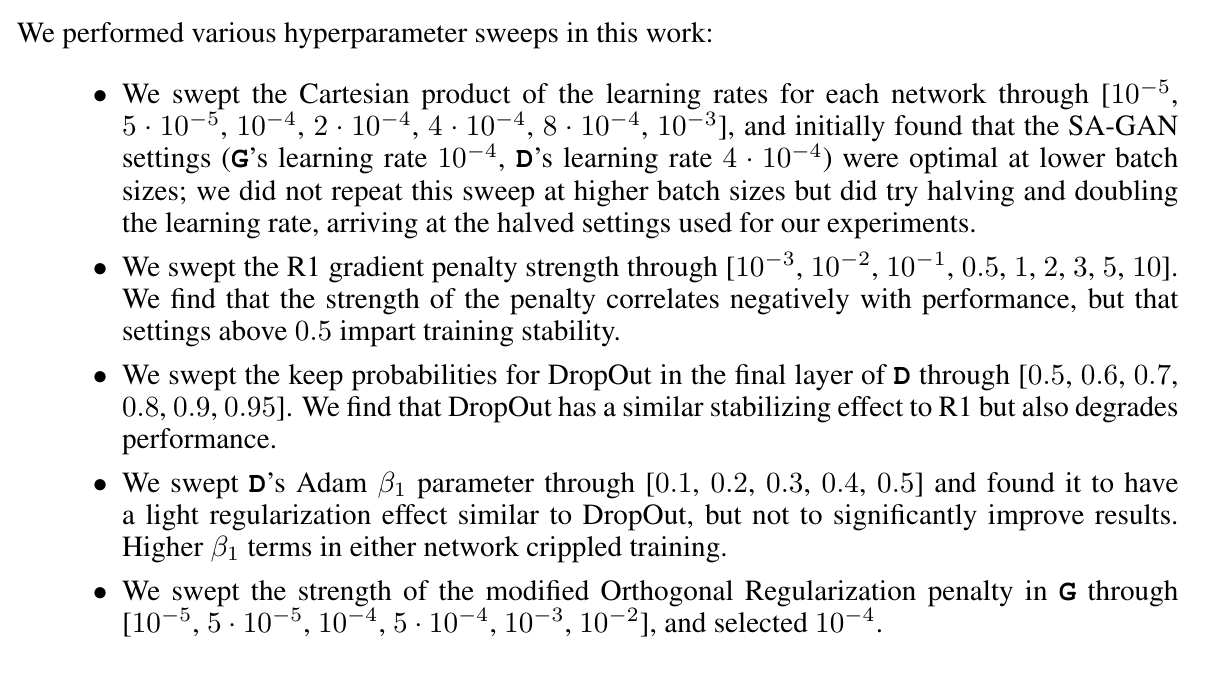
\includegraphics[width=0.6\textwidth]{images/biggan_results_5.png}}

\end{frame}

\begin{frame}{Representation learning benefit from scaling: BigBiGAN}
\protect\hypertarget{representation-learning-benefit-from-scaling-bigbigan}{}

\begin{itemize}
\tightlist
\item
  BigBiGAN(Donahue and Simonyan 2019) asked the following question: can
  GANs learn a useful general representation from unlabeled data ?
\item
  Can we learn high level concepts that we can exploit for downstream
  tasks ?
\end{itemize}

\end{frame}

\begin{frame}{Representation learning benefit from scaling: BigBiGAN}
\protect\hypertarget{representation-learning-benefit-from-scaling-bigbigan-1}{}

\begin{itemize}
\tightlist
\item
  Similar to BigGAN but in addition to discriminator and generator, we
  also have an \textbf{encoder}
\item
  Three networks to optimize simultanously
\end{itemize}

\center{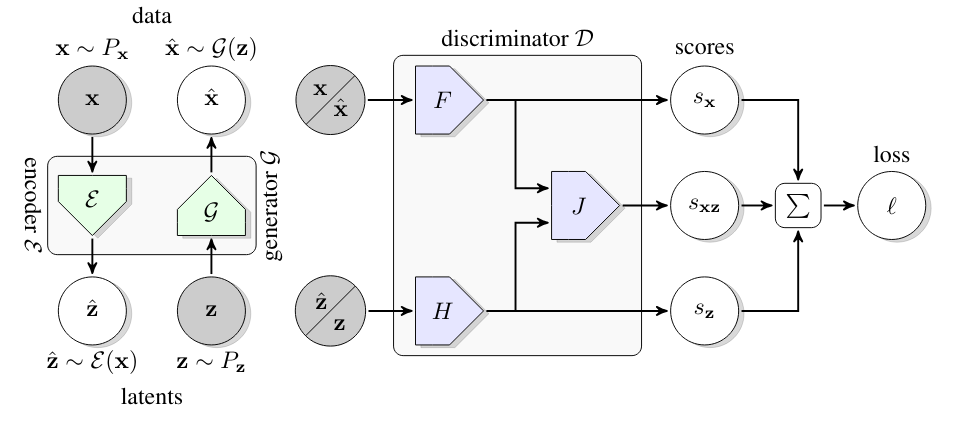
\includegraphics[width=0.8\textwidth]{images/bigbigan_1.png}}

\end{frame}

\begin{frame}{Representation learning benefit from scaling: BigBiGAN}
\protect\hypertarget{representation-learning-benefit-from-scaling-bigbigan-2}{}

\begin{itemize}
\tightlist
\item
  Training on ImageNet-1K up to 256x256 resolution, completely
  unsupervised (no conditioning)
\item
  Training on 32 to 512 TPU cores
\item
  Batch size of 2048 similar to BigGAN
\item
  Architecture similar to BigGAN for \textbf{generator} and
  \textbf{discriminator}, for \textbf{encoder} architecture is based on
  ResNet-50
\end{itemize}

\center{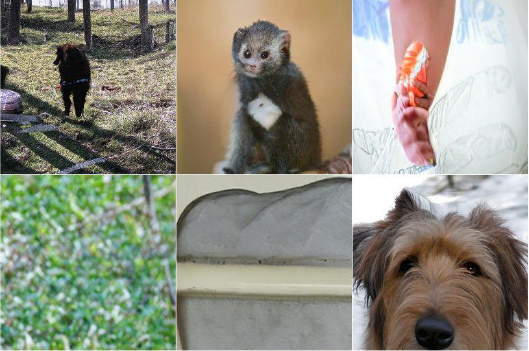
\includegraphics[width=0.4\textwidth]{images/bigbigan_5.png}}

\end{frame}

\begin{frame}{Representation learning benefit from scaling: BigBiGAN}
\protect\hypertarget{representation-learning-benefit-from-scaling-bigbigan-3}{}

\begin{itemize}
\tightlist
\item
  Learned representation focus on high-level semantic details
\end{itemize}

\center{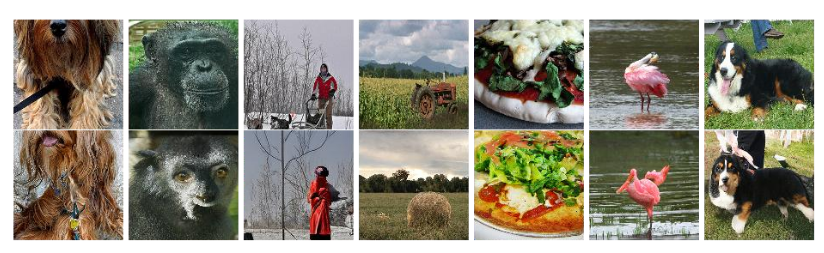
\includegraphics[width=0.6\textwidth]{images/bigbigan_3.png}}

\center{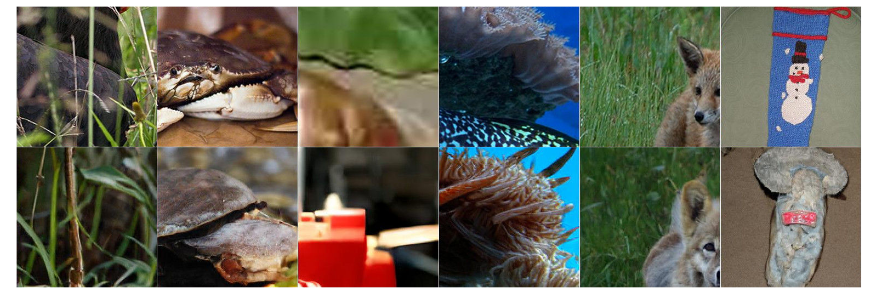
\includegraphics[width=0.6\textwidth]{images/bigbigan_4.png}}

\end{frame}

\begin{frame}{Representation learning benefit from scaling: BigBiGAN}
\protect\hypertarget{representation-learning-benefit-from-scaling-bigbigan-4}{}

\begin{itemize}
\tightlist
\item
  Better image modeling (FID) translates to better performance in
  downstream task (supervised classification)
\item
  Bigger models perform \textbf{better} in downstream task (supervised
  classification)
\end{itemize}

\center{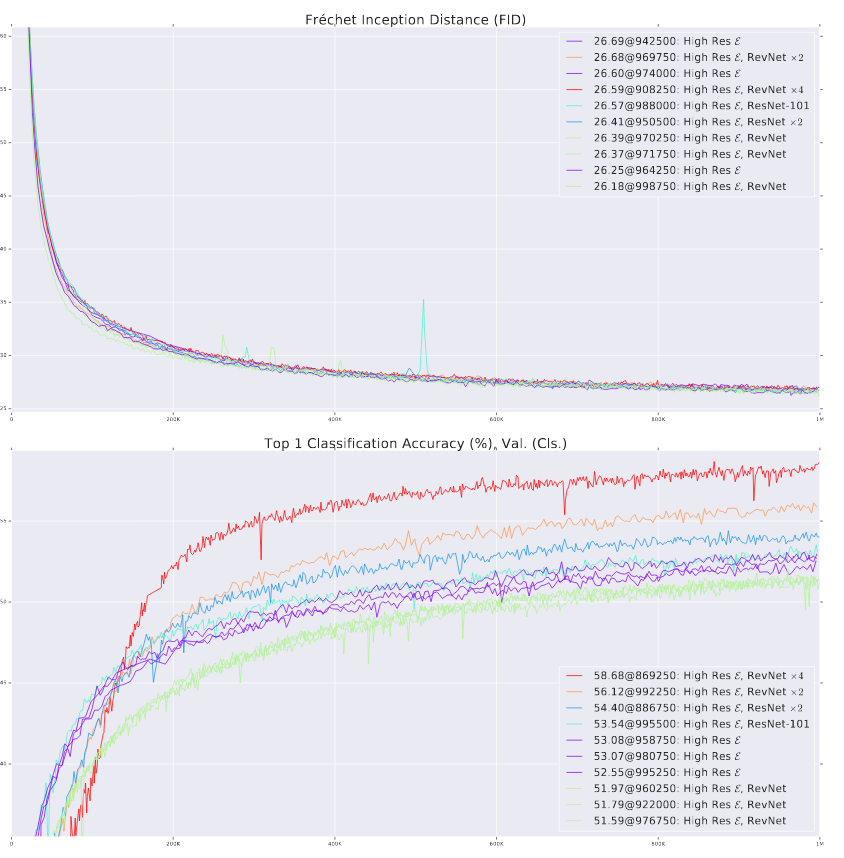
\includegraphics[width=0.34\textwidth]{images/bigbigan_2.png}}

\end{frame}

\begin{frame}{Innovations in architecture: StyleGAN2}
\protect\hypertarget{innovations-in-architecture-stylegan2}{}

\begin{itemize}
\tightlist
\item
  StyleGAN/StyleGAN2 (Karras et al. 2020) introduces a novel way to
  structure the generator architecture
\item
  It decomposes the latent space into \textbf{high level attributes}
  (encoding concepts such pose and identity) and \textbf{stochastic
  variation} (e.g., to handle freckles and hair)
\end{itemize}

\center{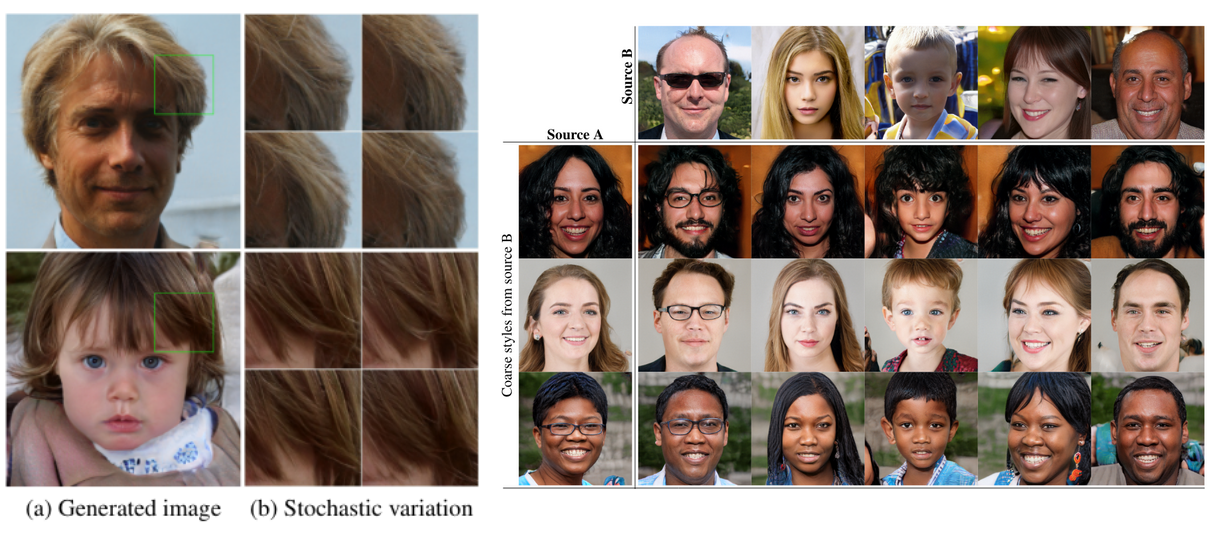
\includegraphics[width=0.8\textwidth]{images/stylegan_representation.png}}

\end{frame}

\begin{frame}{Innovations in architecture: StyleGAN2}
\protect\hypertarget{innovations-in-architecture-stylegan2-1}{}

\begin{itemize}
\tightlist
\item
  The latent \(\boldsymbol{z}\) is converted to
  \(\boldsymbol{w} = f(\boldsymbol{z})\) using 8 fully connected layers
  \(f\)
\item
  The \(\boldsymbol{w}\) vector is then mapped to a style vector using a
  fully connected network for each resolution. One style vector per
  resolution.
\end{itemize}

\center{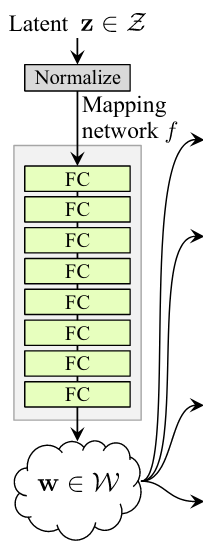
\includegraphics[width=0.13\textwidth]{images/stylegan_latent_space.png}}

\end{frame}

\begin{frame}{Innovations in architecture: StyleGAN2}
\protect\hypertarget{innovations-in-architecture-stylegan2-2}{}

\begin{itemize}
\tightlist
\item
  One block per resolution, each block upsample by 2
\item
  Each resolution block is affected by its dedicated style vector \(A\)
  and noise \(B\)
\end{itemize}

\center{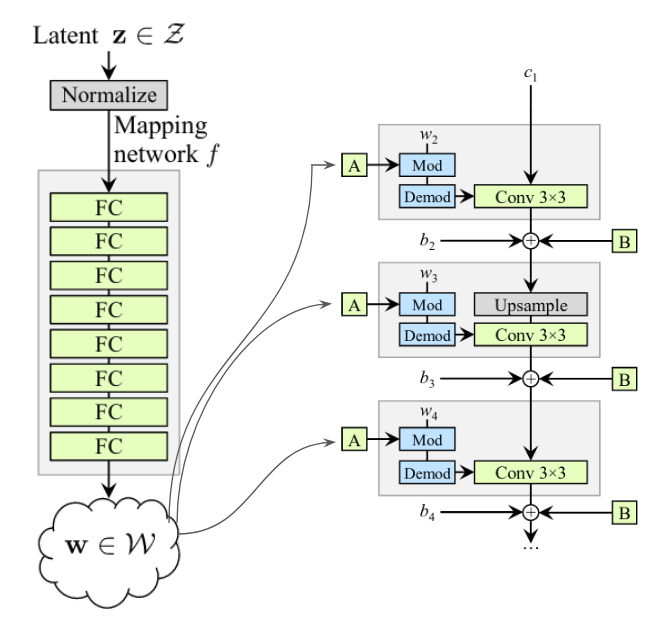
\includegraphics[width=0.4\textwidth]{images/stylegan2.png}}

\end{frame}

\begin{frame}{Innovations in architecture: StyleGAN2}
\protect\hypertarget{innovations-in-architecture-stylegan2-3}{}

\begin{itemize}
\tightlist
\item
  No need progressive generation like in ProGAN (Karras et al. 2018)
\item
  The generated image RGBs are a sum of RGBs from each resolution
  outputs, everything is learned simultanously
\end{itemize}

\center{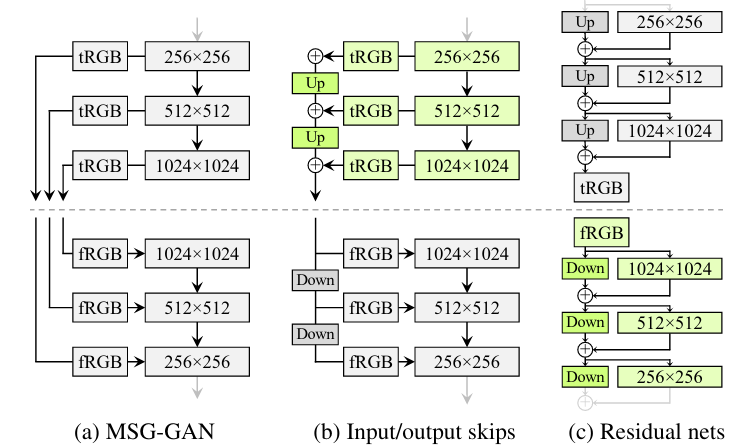
\includegraphics[width=0.7\textwidth]{images/stylegan_output.png}}

\end{frame}

\begin{frame}{Innovations in architecture: StyleGAN2}
\protect\hypertarget{innovations-in-architecture-stylegan2-4}{}

\begin{itemize}
\tightlist
\item
  Larger configuration network renders high resolution details better
\end{itemize}

\center{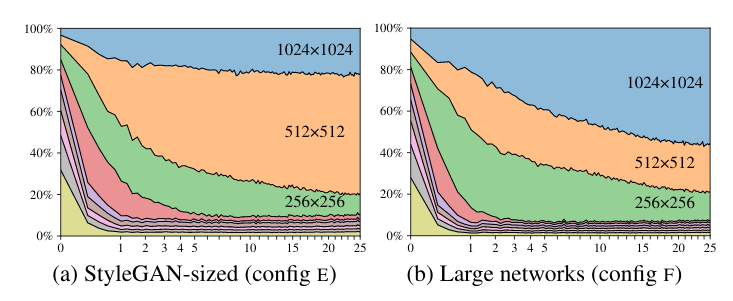
\includegraphics[width=0.8\textwidth]{images/stylegan_large.png}}

\end{frame}

\begin{frame}{Innovations in architecture: StyleGAN2}
\protect\hypertarget{innovations-in-architecture-stylegan2-5}{}

\begin{itemize}
\tightlist
\item
  Distributed training on 8 V100 GPUs
\item
  Reduce training time from 70 days with 1 GPU to 10 days with 8 GPUs
\end{itemize}

\center{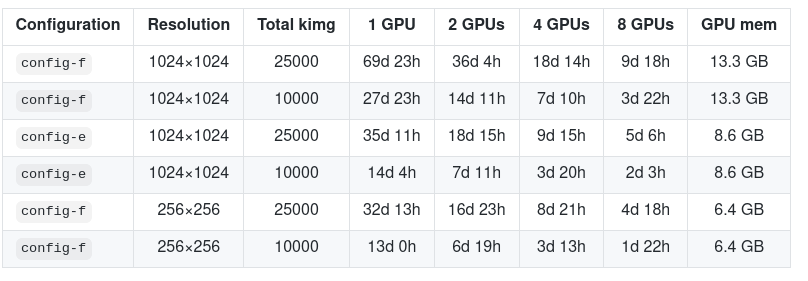
\includegraphics[width=0.8\textwidth]{images/stylegan_time.png}}

\end{frame}

\begin{frame}{Innovations in architecture: StyleGAN2}
\protect\hypertarget{innovations-in-architecture-stylegan2-6}{}

\begin{itemize}
\tightlist
\item
  One should not forget the cost of exploration as well: 51 GPU years
  was required in total
\end{itemize}

\center{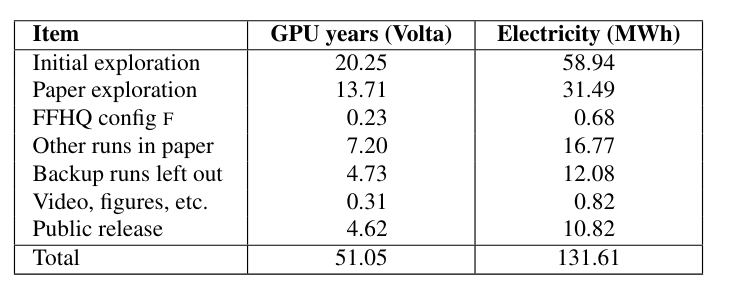
\includegraphics[width=0.8\textwidth]{images/stylegan_gpuyears.png}}

\end{frame}

\begin{frame}{StyleGAN-XL: Scaling StyleGAN to Large Diverse Datasets}
\protect\hypertarget{stylegan-xl-scaling-stylegan-to-large-diverse-datasets}{}

\begin{itemize}
\tightlist
\item
  Up until now, StyleGAN models had difficulties with large diverse
  datasets such as ImageNet
\item
  By combining different techniques, StyleGAN-XL (Sauer, Schwarz, and
  Geiger 2022) could achieve state of the art results on ImageNet for
  the first time
\end{itemize}

\center{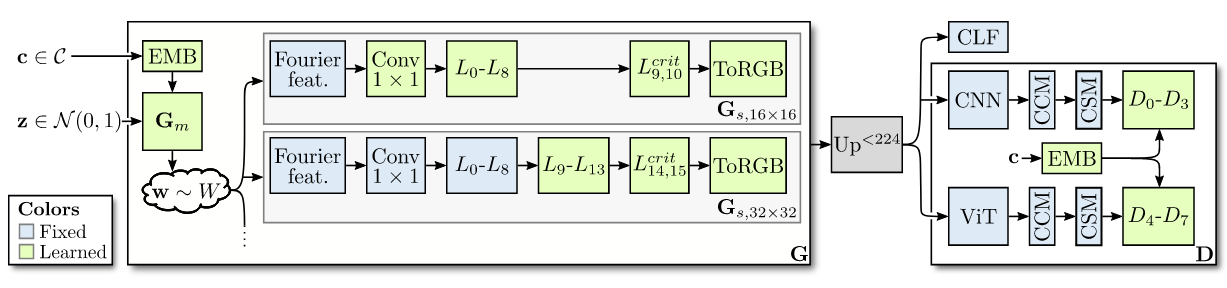
\includegraphics[width=0.8\textwidth]{images/stylegan-xl.png}}

\end{frame}

\begin{frame}{StyleGAN-XL: Scaling StyleGAN to Large Diverse Datasets}
\protect\hypertarget{stylegan-xl-scaling-stylegan-to-large-diverse-datasets-1}{}

\begin{itemize}
\tightlist
\item
  They leverage several recent techniques to improve sample quality
\item
  In particular, they exploit the rich representation of several
  pre-trained models (supervised and self-supervised)
\end{itemize}

\center{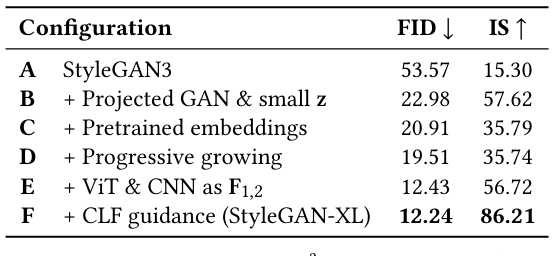
\includegraphics[width=0.8\textwidth]{images/stylegan-xl-ablation.png}}

\end{frame}

\begin{frame}{Innovations in architecture: GANsFormer}
\protect\hypertarget{innovations-in-architecture-gansformer}{}

\begin{itemize}
\tightlist
\item
  StyleGAN2 have been shown to have difficulties with datasets with a
  lot of diversity, e.g., complex scenes with multiple objects
\item
  This is possibly attributed to the fact that one global latent
  controls all the styles simultanously
\item
  GANsFormer (Hudson and Zitnick 2021) is a new architecture, based on
  StyleGAN2, where they have multiple latents and use transformers to
  integrate information from the latents into the image
\end{itemize}

\end{frame}

\begin{frame}{Innovations in architecture: GANsFormer}
\protect\hypertarget{innovations-in-architecture-gansformer-1}{}

\begin{itemize}
\tightlist
\item
  we have multiple latents instead of a single one that globally
  controls the image
\end{itemize}

\center{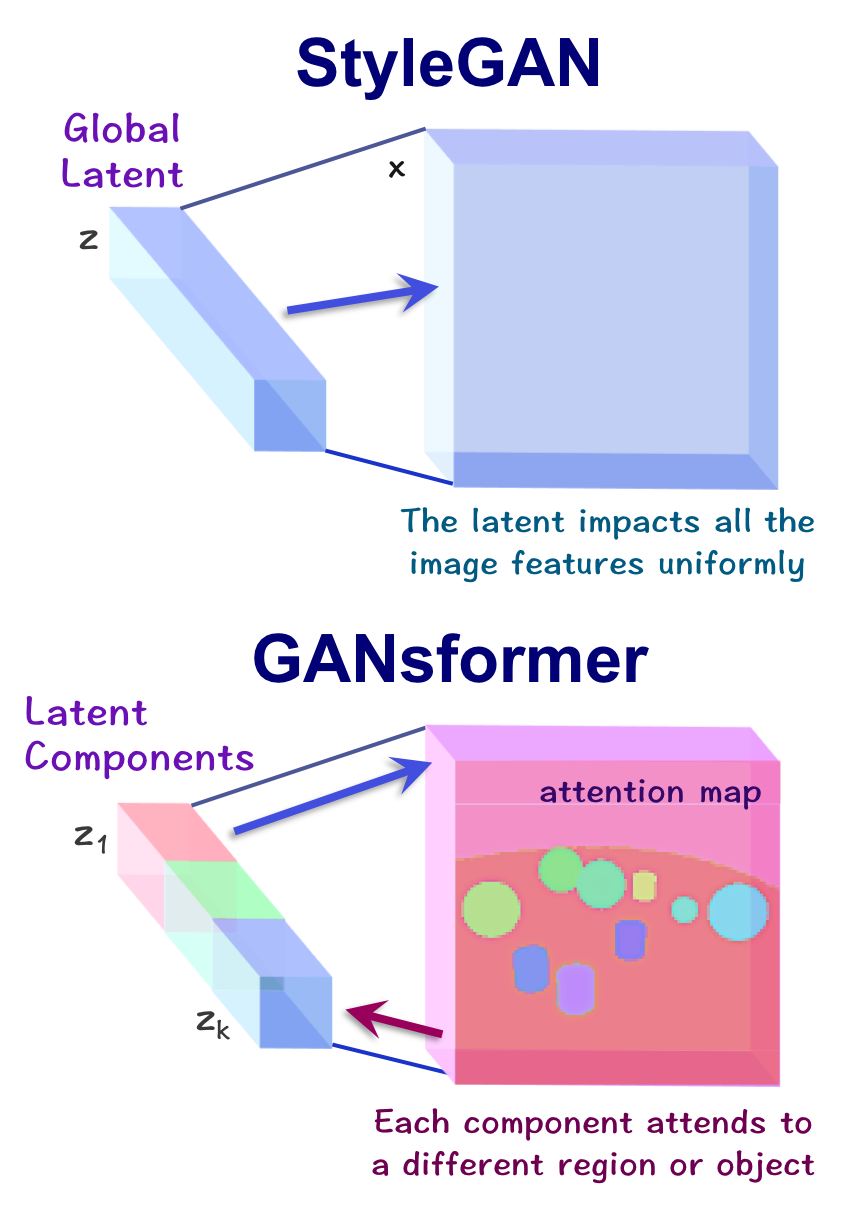
\includegraphics[width=0.33\textwidth]{images/gansformer1.png}}

\end{frame}

\begin{frame}{Innovations in architecture: GANsFormer}
\protect\hypertarget{innovations-in-architecture-gansformer-2}{}

\begin{itemize}
\tightlist
\item
  To integrate information from the latents \(Y\) into the image \(X\),
  they use a transformer architecture
\item
  To make the transformer efficient, they use a bipartite structure,
  where connections are made between image features and latents only
\end{itemize}

\center{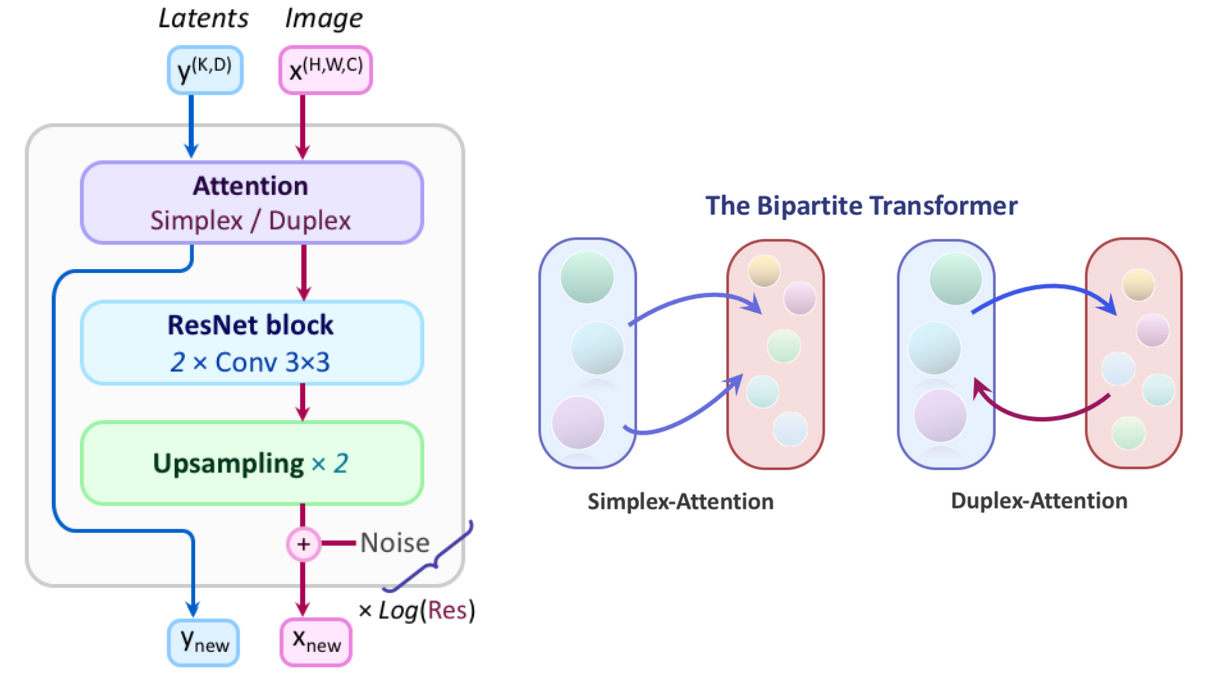
\includegraphics[width=0.6\textwidth]{images/gansformer6.png}}

\end{frame}

\begin{frame}{Innovations in architecture: GANsFormer}
\protect\hypertarget{innovations-in-architecture-gansformer-3}{}

\begin{itemize}
\tightlist
\item
  Different latents specialize in different aspects of the image
\end{itemize}

\center{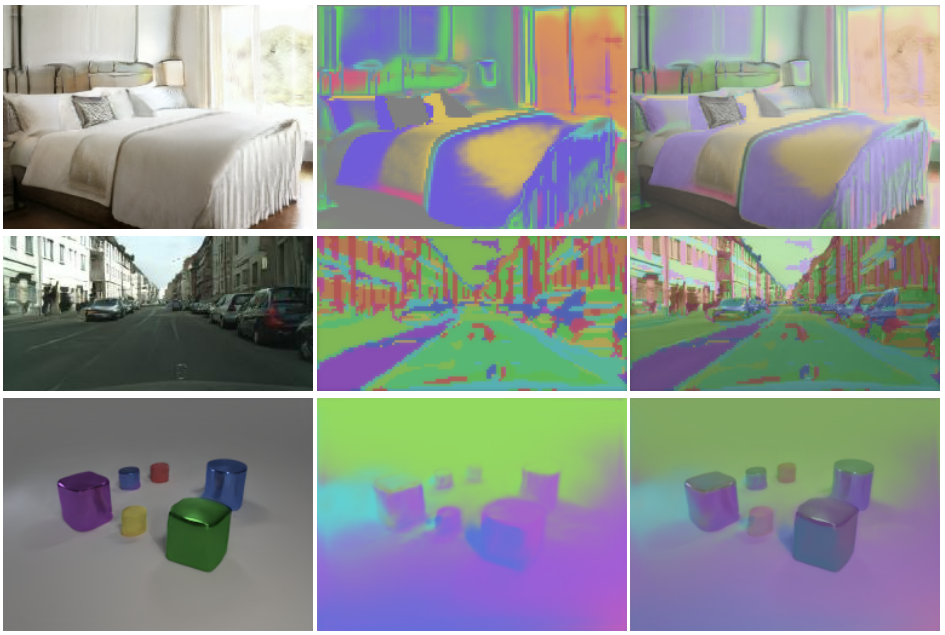
\includegraphics[width=0.75\textwidth]{images/gansformer3.png}}

\end{frame}

\begin{frame}{Summary}
\protect\hypertarget{summary}{}

\begin{itemize}
\tightlist
\item
  We have seen different architectures proposed in the literature
\item
  The GANs are in general costly to train, especially with larger
  resolutions and for large datasets.
\item
  Distributed training helps to make training faster
\end{itemize}

\end{frame}

\begin{frame}[allowframebreaks]{References}
\protect\hypertarget{references}{}

\hypertarget{refs}{}
\leavevmode\hypertarget{ref-brock2019large}{}%
Brock, Andrew, Jeff Donahue, and Karen Simonyan. 2019. ``Large Scale Gan
Training for High Fidelity Natural Image Synthesis.''
\url{http://arxiv.org/abs/1809.11096}.

\leavevmode\hypertarget{ref-donahue2019large}{}%
Donahue, Jeff, and Karen Simonyan. 2019. ``Large Scale Adversarial
Representation Learning.'' \url{http://arxiv.org/abs/1907.02544}.

\leavevmode\hypertarget{ref-hudson2021generative}{}%
Hudson, Drew A, and C Lawrence Zitnick. 2021. ``Generative Adversarial
Transformers.'' \emph{arXiv Preprint arXiv:2103.01209}.

\leavevmode\hypertarget{ref-karras2018progressive}{}%
Karras, Tero, Timo Aila, Samuli Laine, and Jaakko Lehtinen. 2018.
``Progressive Growing of Gans for Improved Quality, Stability, and
Variation.'' \url{http://arxiv.org/abs/1710.10196}.

\leavevmode\hypertarget{ref-karras2020training}{}%
Karras, Tero, Miika Aittala, Janne Hellsten, Samuli Laine, Jaakko
Lehtinen, and Timo Aila. 2020. ``Training Generative Adversarial
Networks with Limited Data.'' \url{http://arxiv.org/abs/2006.06676}.

\leavevmode\hypertarget{ref-sauer2022stylegan}{}%
Sauer, Axel, Katja Schwarz, and Andreas Geiger. 2022. ``StyleGAN-Xl:
Scaling Stylegan to Large Diverse Datasets.'' \emph{arXiv Preprint
arXiv:2202.00273}.

\end{frame}


\end{document}
